\documentclass[parskip]{scrartcl}
\usepackage[margin=15mm]{geometry}
\usepackage{tikz}
\usetikzlibrary{shadings}

\begin{document}
	
	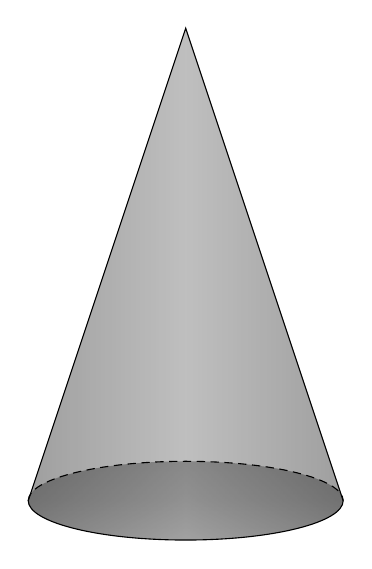
\begin{tikzpicture}
	\fill[top color=gray!50!black,bottom color=gray!10,middle color=gray,shading=axis,opacity=0.25] (0,0) circle (2cm and 0.5cm);
	\fill[left color=gray!50!black,right color=gray!50!black,middle color=gray!50,shading=axis,opacity=0.25] (2,0) -- (0,6) -- (-2,0) arc (180:360:2cm and 0.5cm);
	\draw (-2,0) arc (180:360:2cm and 0.5cm) -- (0,6) -- cycle;
	\draw[densely dashed] (-2,0) arc (180:0:2cm and 0.5cm);
	\end{tikzpicture}
	\hspace{1cm}
	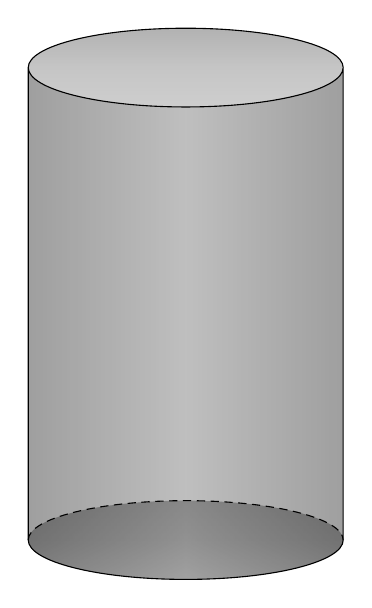
\begin{tikzpicture}
	\fill[top color=gray!50!black,bottom color=gray!10,middle color=gray,shading=axis,opacity=0.25] (0,0) circle (2cm and 0.5cm);
	\fill[left color=gray!50!black,right color=gray!50!black,middle color=gray!50,shading=axis,opacity=0.25] (2,0) -- (2,6) arc (360:180:2cm and 0.5cm) -- (-2,0) arc (180:360:2cm and 0.5cm);
	\fill[top color=gray!90!,bottom color=gray!2,middle color=gray!30,shading=axis,opacity=0.25] (0,6) circle (2cm and 0.5cm);
	\draw (-2,6) -- (-2,0) arc (180:360:2cm and 0.5cm) -- (2,6) ++ (-2,0) circle (2cm and 0.5cm);
	\draw[densely dashed] (-2,0) arc (180:0:2cm and 0.5cm);
	\end{tikzpicture}
	
\end{document}
